\documentclass{beamer}

\usepackage[T2A]{fontenc}
\usepackage[utf8]{inputenc}
\usepackage[russian]{babel}
\usepackage{graphicx}

\usetheme{Madrid}
\usecolortheme{whale}

\hypersetup {
    unicode = true
}

\title[]{Инструментальная среда для анализа программных систем}
\author[А.М. Полоцев]{
    А.М. Полоцев, гр. 63501/13\\
    научный руководитель: к.т.н. доцент В.М. Ицыксон
}
\date[XLII Неделя науки]{XLII Неделя науки}

\begin{document}
%===============================================================================
\frame{\titlepage}
%===============================================================================
%===============================================================================
\begin{frame}
\frametitle{Постановка задачи}

\begin{itemize}
    \item В различных методах анализа часто решаются похожие задачи:
    \begin{itemize}
        \item Построение моделей программы (AST, CFG и т.п.)
        \item Построение метрик
        \item Реинжиниринг программного обеспечения (оптимизация, рефакторинг и т.п.)
        \item Визуализация свойств системы
    \end{itemize}
    \item Обычно эти задачи решаются вручную
\end{itemize}
\end{frame}
%===============================================================================
%===============================================================================
\begin{frame}
\frametitle{Разработка инструментального средства}

\begin{itemize}
    \item Цели
        \begin{itemize}
            \item Автоматизация анализа
            \item Визуализация свойств системы
        \end{itemize}
    \item Требования
        \begin{itemize}
            \item Тут будут требования
        \end{itemize}
\end{itemize}
\end{frame}
%===============================================================================
%===============================================================================
\begin{frame}
\frametitle{Архитектура инструментального средства}

\begin{figure}[h!]
    \begin{center}
        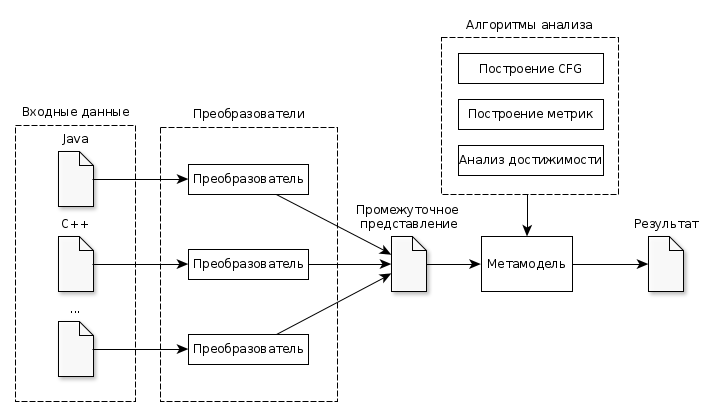
\includegraphics[width=\textwidth]{img/architecture.png}
    \end{center}
\end{figure}
\end{frame}
%===============================================================================
%===============================================================================
\begin{frame}[t]
\frametitle{Разработка метамодели}


\end{frame}
%===============================================================================
%===============================================================================

\end{document}
